% Author: Pavel Semenov
% Date: 17.01.2023

\documentclass{article}
\usepackage{array}
\usepackage{longtable}
\usepackage{float}
\usepackage{graphicx}
\usepackage{amsmath}
\usepackage{listings}
\usepackage{xcolor}
\usepackage{hyperref}

\hypersetup{
    colorlinks=true,
    linkcolor=blue,
    filecolor=magenta,      
    urlcolor=cyan,
}

\definecolor{codegreen}{rgb}{0,0.6,0}
\definecolor{codegray}{rgb}{0.5,0.5,0.5}
\definecolor{codepurple}{rgb}{0.58,0,0.82}
\definecolor{backcolour}{rgb}{0.95,0.95,0.92}
\definecolor{codedarkblue}{rgb}{0.11,0.13,0.5}

\lstdefinestyle{mystyle}{
    backgroundcolor=\color{backcolour},   
    commentstyle=\color{codegreen},
    keywordstyle=\color{magenta},
    numberstyle=\tiny\color{codegray},
    stringstyle=\color{codepurple},
    basicstyle=\ttfamily\color{codedarkblue},
    breakatwhitespace=false,         
    breaklines=true,                 
    captionpos=b,                    
    keepspaces=true,                 
    numbers=left,                    
    numbersep=5pt,                  
    showspaces=false,                
    showstringspaces=false,
    showtabs=false,                  
    tabsize=2
}

\lstset{language=Python,style=mystyle}
\graphicspath{ {./figures/} }
\setlength{\parindent}{0pt}
\AddToHook{cmd/section/before}{\clearpage}

\title{Project for Machine Learning 2022/2023}
\author{Pavel Semenov}
\date{17.01.2023}
\begin{document}
\maketitle

\section{Introduction}
One of the biggest headaches of the project managers is accurate effort estimates.
Good estimates allow to organize project work more efficiently and plan budget more precisely, thus, saving money.
While an experienced project manager is able to render an estimate from the task parameters with no issues, it might
be hard for employees from other roles to do the same. In this document I describe my attempts to produce a model,
which is able to give an estimation of time required to resolve a work item based on its parameters. Though the initial
was not achieved, my experiments included several iterations of trials with different tools, libraries and techniques,
which might be worth documenting.

\section{Dataset}
My dataset is, basically, an export file from the project management system. It consists of \textbf{28791} work items 
and each of them has a few poperties, which in my opinion might influence he time spent on the task. Here is an example
of one work item:
\begin{center}
    \begin{longtable}[H]{ | m{5em} | m{10em}| m{20em} | }  
        \hline
        Name & Description & Example \\
        \hline\hline
        timeSpent & The time spent on the task in milliseconds & 144000000 \\
        \hline
        summary & Short summary of the work item & FST-4320 - Falscher Ablauf beim Versand XJustiz Nachricht \\
        \hline
        description & Multiline description of the work item & 
        Es existiert ein FAM VA Verfahren mit Auskunftsersuchen. Eine XJustiz Nachricht nachricht.vag.fehler Version 3.3.1 mit Signaturstatus unknown, mit fehlerhafte Schematronprüfung und erfolgreiche Plausibilitätsprüfung wurde an Postfach gesendet.
        Es läuft der AF002 Normalablauf (Schritte 1-9). Im Schritt 10. stellt System fest, dass Regelverstöße bei der Schematronprüfung vorliegen. \\
        \hline
        priority & Priority assigned to the work item. Ranged from 1 to 5 & Prio 2 \\
        \hline
        severity & The severity of the work item. Blocker, Normal, Minor, Major, Critical are some of the values. (fixed collection of values) & Blocker \\
        \hline
        category & Category of the work item. Might be Release-Test, KM, Maintenance, etc. (fixed collection of values) & Release-Test \\
        \hline
        type & Type of the work item. Internal Defect/Issue/Action/etc. (fixed collection of values) & Issue \\
        \hline
\end{longtable}
\end{center}
    
\section{Data pre-processing}
Since the raw data is in the \textbf{XML} format, I decided to parse it into the common format, where the samples
are separated by the line breaks and the features are separated by the spaces. This stage also includes encoding
the text data into the vector form.

\subsection{Feature encoding}
Since most of the features are represented by a static set of values, I have enumerated those values in such way,
that unassigned values are turned to zeroes. Here I have experimented with feature scaling. Three methods were tested:
no feature scaling, normalization and standardization. Normalization (scaling between $0$ and $1$) was obtained by
using the following equation:
\[ x' = \frac{x - \min (x)}{\max (x) - \min (x)} \]
However, normalization gave slightly worse results compared to the model without any feature scaling applied. 
Standardization of features has been computed with the equation below:
\[ x' = \frac{x - \bar x}{\sigma} \]
Here $\sigma$ is a standard deviation, which is calculated as
\[ \sigma = \sqrt \frac{\sum (x_i - \mu)^2}{N} \]
Standardization has shown even worse results as it also has scaled some features into infinity.
The results are plotted as bar chart (see Figure~\ref{fig:Figure_1}). It is clear that no feature scaling
is required for this dataset, so all further experiments are conducted without feature scaling.

\begin{figure}[h!]
    \centering
    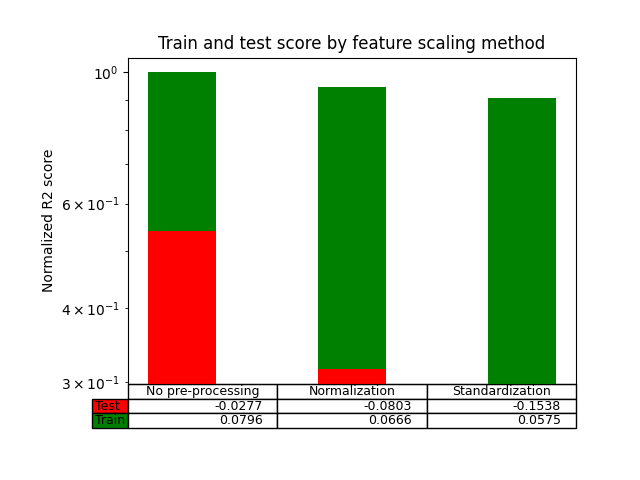
\includegraphics[width=0.8\textwidth]{Figure_1.png}
    \caption{Comparison of feature scaling techniques in terms of $R2$ score. Y axis has normalized $R2$ score, 
    whereas the bottom table presents raw values.}\label{fig:Figure_1}
\end{figure}

\subsection{Text encoding}
Before vectorizing the text it is important to deprive it of every undesired details. Therefore, I am removing
all special characters and numbers from the text prior to vectorizing it. The following function is designed to do so:

\begin{lstlisting}
def clean(text):
    return re.sub("[^a-zA-Z0-9 ]+", '', text)
\end{lstlisting}

I have conducted experiments with two modules: the \lstinline{sklearn.feature_extraction.text}, from which I am 
using \lstinline{CountVectorizer} class, and the \lstinline{fasttext}, which is developed and maintained by Facebook.
The former (as suggested by its name) encodes the text into a vector with the number of features equal to the 
vocabulary size found by analyzing the data, and each feature is a count of occurences of the word in the input text. 
The latter obtains the vector reprezentation using either unsupervised or supervised learning. When using \lstinline{CountVectorizer}
we have two options: either feed it a precomposed vocabulary to work with or let it learn the vocabulary of the whole
text input. The first option should, in theory, yield better results, but it requires some method of extracting 
words, which have the most influence on the outcome. I did not manage to find a way to compose a good vocabulary and
had to utilize the second option instead. Thus, I ended up with almost $300k$ features, most of which were zeroes.
That is when I came up with idea to reduce the dimensionality of the input using feature selection methods (I describe
them in the next section). \\ \\
Another big advantage of \lstinline{fasttext} is its perfomance. \lstinline{CountVectorizer} does not have an option to 
save and reuse model and, therefore, we have to retrain it every time we want to render an input file.\lstinline{fasttext},
on the other hand, does offer this option, allowing to generate a binary file with pretrained model, which is then loaded
from the script. So in this test we are comparing the results of the four models: model using \lstinline{fasttext}
without the feature selection, model using \lstinline{fasttext} with feature selection, model using \lstinline{CountVectorizer} without the
feature selection and \lstinline{CountVectorizer} with feature selection (see Figure~\ref{fig:Figure_2}). The test had
to be perfomed on $100$ samples only (instead of the common $1000$) as anything above lead my laptop to freezing.
According to the plot, both variants of \lstinline{fasttext} have the same perfomance score. This is caused by feature selection
not changing the feature vector on such small sample size. However, when considering \lstinline{CountVectorizer}
we can see a big perfomance improvment in terms of test score when feature selection is applied. Interestingly, 
when using \lstinline{CountVectorizer} without the feature selection, score on the training set greatly bigger
than on the test set, which means huge overfit. With feature selection, though, those $300k$ features are reduced 
to around $20$ with $C=0.1$. Nevertheless, \lstinline{fasttext} still outperforms \lstinline{CountVectorizer} and 
is better in multiple ways described before, thus, we will be using it in all our forthmentioned experiments. 

\begin{figure}[H]
    \centering
    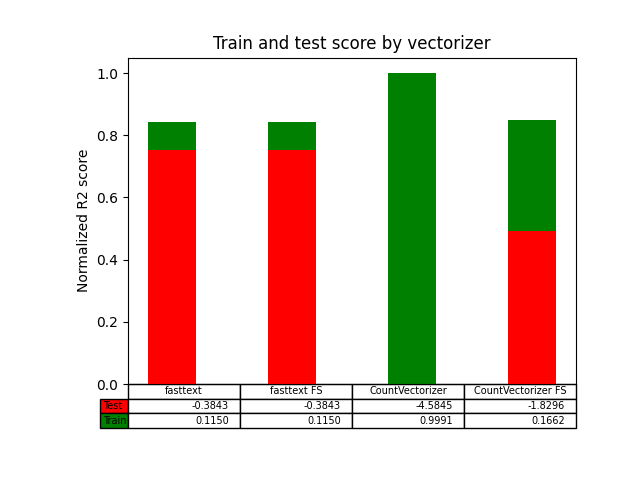
\includegraphics[width=0.8\textwidth]{Figure_2.png}
    \caption{Comparison of text vectorizing techniques in terms of $R2$ score. Y axis has normalized $R2$ score, 
    whereas the bottom table presents raw values.}\label{fig:Figure_2}
\end{figure}


\section{Feature selection}
I am using \lstinline{sklearn.svm.LinearSVC} with $l1$ penalty as a feature selection method. This is a piece
of code, which performs feature selection:

\begin{lstlisting}
def feature_selection(X, y, C=0.01, max_iter=1000):
    lsvc = LinearSVC(C=C, penalty="l1", dual=False, max_iter=max_iter).fit(X, y)
    model = SelectFromModel(lsvc, prefit=True)
    return model.transform(X)
\end{lstlisting}

Here we are tweaking \lstinline{C} parameter to find the best results. Feature selection
doesn't really influence the perfomance when using \lstinline{fasttext}, so these experiments were conducted using
the \lstinline{CountVectorizer} instead. Increasing $C$
corresponds to less regularization and vice versa. The graph below (see Figure~\ref{fig:Figure_3}) depicts the 
results of experiments with different values of $C$. It looks like the value of $0.3$ has the best scores. Everything
below $0.25$ does not leave enough features for the regression, and after $1.2$ we have too much features left.

\begin{figure}[h!]
    \centering
    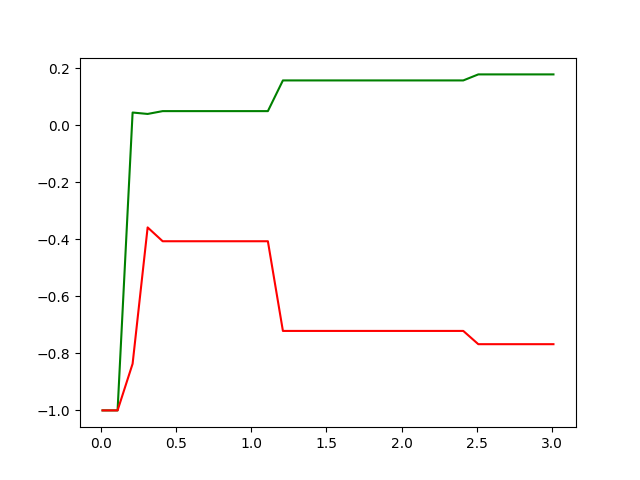
\includegraphics[width=0.8\textwidth]{Figure_3.png}
    \caption{Comparison of different regularization values in feature selection.
    The red curve is test score and the green one is the train score.}\label{fig:Figure_3}
\end{figure}

There is no point tweaking \lstinline{max_iter} since \lstinline{LinearSVC} converges before it reaches $1000$ iterations,
so it yields the same results for every other number of iterations above that value. And decreasing the number of iterations
leads to non-convergence, which is not exactly what we want. 

\section{Model tuning}
Now that we have chosen a text vectorizer we can compare different models. \lstinline{Sckit-learn} library has a few
linear models implemented. Some of them, like for instance \lstinline{Lasso}, already include variable selection in them.
There is also \lstinline{LassoCV} with $k$-fold cross validation, which we can use to find optimal model for us.
In this section we are comparing different models, such as \lstinline{LinearRegression}, \lstinline{LinearRegression+LinearSVC},
\lstinline{LassoCV}. According to the Figure~\ref{fig:Figure_4}, the overall best results were achieved when using \lstinline{LassoCV}.
Bare linear regression is very exposed to overfitting on the undesired features. When using \lstinline{LinearSVC} to select features,
and then feeding reduced feature vector to the \lstinline{LinearRegression} we get interesting results: ahieved test score is 
bigger than the train score.

\begin{figure}[H]
    \centering
    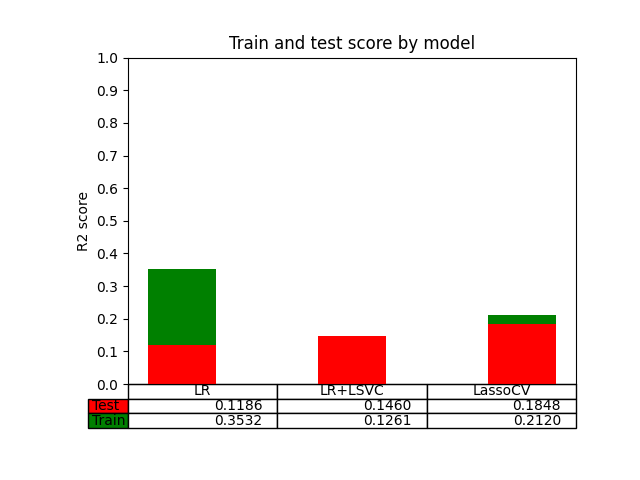
\includegraphics[width=0.8\textwidth]{Figure_4.png}
    \caption{Comparison of different models.
    }\label{fig:Figure_4}
\end{figure}

\lstinline{LassoCV} is actually yielding some adequate results, though, of course I was aiming for more initially.
To better understand how good is it performing, here are a few sample results:
\begin{lstlisting}
got: 68864.5, expected: 59400.0
got: 38284.0, expected: 7200.0
got: 20963.4, expected: 1800.0
got: 186710.0, expected: 144000.0
got: 54440.0, expected: 10800.0
\end{lstlisting}

\section{Conclusion}
All in all, after multiple iterations and experiments I can conclude, that it is very hard to predict the time
estimate based on this (real-world) dataset. After all, the time spent on the task does not only depend on its
priority, severity, description or other parameters, but also on the person, who was the task assigned to. Moreover,
complexity of the task can vary depending on different other conditions not possible to include in the dataset.\\ \\
However, I think there is still a lot of space for research. Firstly, I believe that by generating the right vocabulary
for the \lstinline{CountVectorizer} we can get some satisfiable results from the model. Secondly, the dataset is not
very clean, so it will surely improve the results if we prune it of outliers and exceptions. 
Lastly, other linear regression
models can be researched like \lstinline{Ridge} and \lstinline{SGDRegressor} offered by \textit{scikit-learn} library. \\ \\
Personally, I was really pleased, when I got a test score of $0.18$, but, unfortunately, this is the maximum I could
squeeze out of my models. Additionally, this is the first time I am facing data pre-preprocessing, this project made
me realize how important and how hard it is to clean and prepare your dataset before feeding it to the model.

\section{Appendix}

Source code and other related files can be found in \href{https://github.com/pavel-semenov-1/ml-project-public}{this repository}.
Unfortunately, I did not receive a permission to share the dataset itself as it holds too much corporate data.
However, I think it is rather safe to share the input files, which are created with \lstinline{parse} function.
Repository also contains \textit{model.vec} and \textit{model.bin} files, which hold the \lstinline{fasttext} model.
The \textit{poject.py} is the main script, where I did all my experiments. It is rather messy and has a lot of commented
code, I am attaching it mainly to prove that everything above was computed and generated with the script.

\end{document}